\begin{pa} \label{PA:9.7} Let $\vr(t) = \cos(t) \vi + \sin(2t) \vj$ describe the path traveled by an object at time $t$. 
    \ba

    \item Use appropriate technology to help you sketch the graph of the vector-valued function $\vr(t)$, and then locate and label the point on the graph when $t=\pi$.

    \item Recall that for functions of a single variable, the derivative of a sum is the sum of the derivatives; that is, $\frac{d}{dx}[f(x) + g(x)] = f'(x) + g'(x)$. With this idea in mind and viewing $\vi$ and $\vj$ as constant vectors, what do you expect the derivative of $\vr$ to be?  Write a proposed formula for $\vr'(t)$.

    \item Use your result from part (b) to compute $\vr'(\pi)$. Sketch this vector $\vr'(\pi)$ as emanating from the point on the graph of $\vr$ when $t=\pi$ , and explain what you think $\vr'(\pi)$ tells us about the object's motion.

    \ea

\end{pa} 

\begin{activitySolution}
    \ba
	\item The graph of $\vr(t)$ is shown below, with the point $(-1,0)$ at $t=pi$ indicated as the solid point on the graph. 
\begin{center}
\resizebox{!}{2.0in}{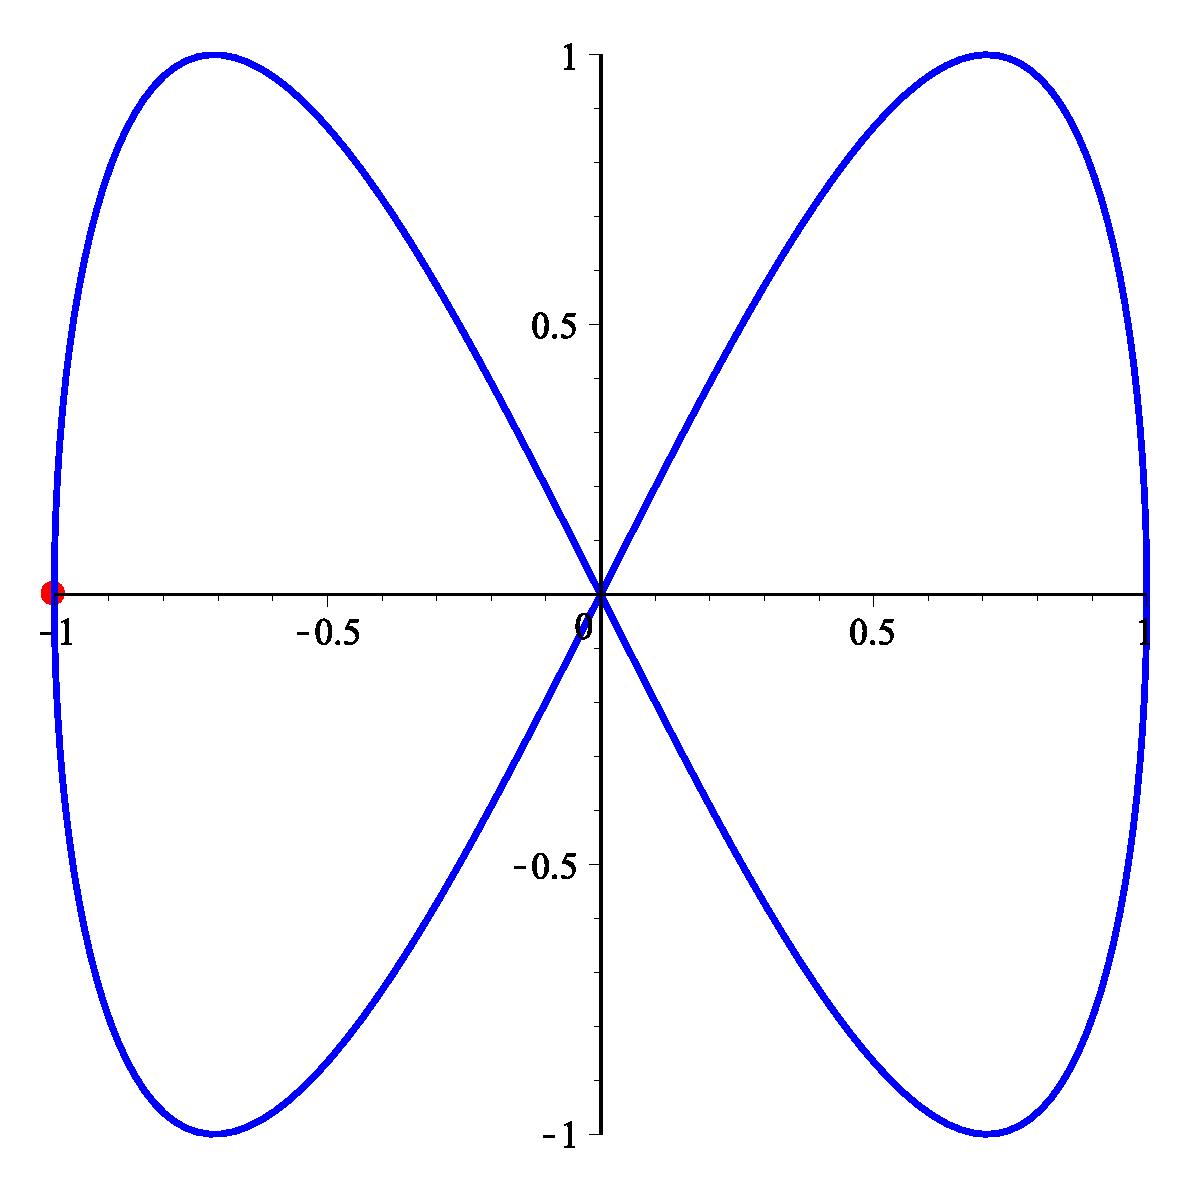
\includegraphics{fig_9_7_PA_a}}
\end{center}

	\item If the derivative of a sum is the sum of the derivatives, then we should expect that 
\[\vr'(t) = \frac{d}{dt} \cos(t) \vi + \frac{d}{dt} \sin(2t) \vj = -\sin(t) \vi + 2\cos(2t) \vj.\]


    \item Using our rule for $\vr'(t)$ we have $\vr'(\pi) = 2 \vj$. A sketch of this vector $\vr'(\pi)$ as emanating from the point on the graph of $\vr$ when $t=\pi$ is shown below. This looks like a direction vector for the line tangent to the graph of $\vr$ at the point where $t = \pi$. In other words, this vector $\vr'(t)$ is the velocity vector of the object at time $t = \pi$. 
\begin{center}
\resizebox{!}{2.0in}{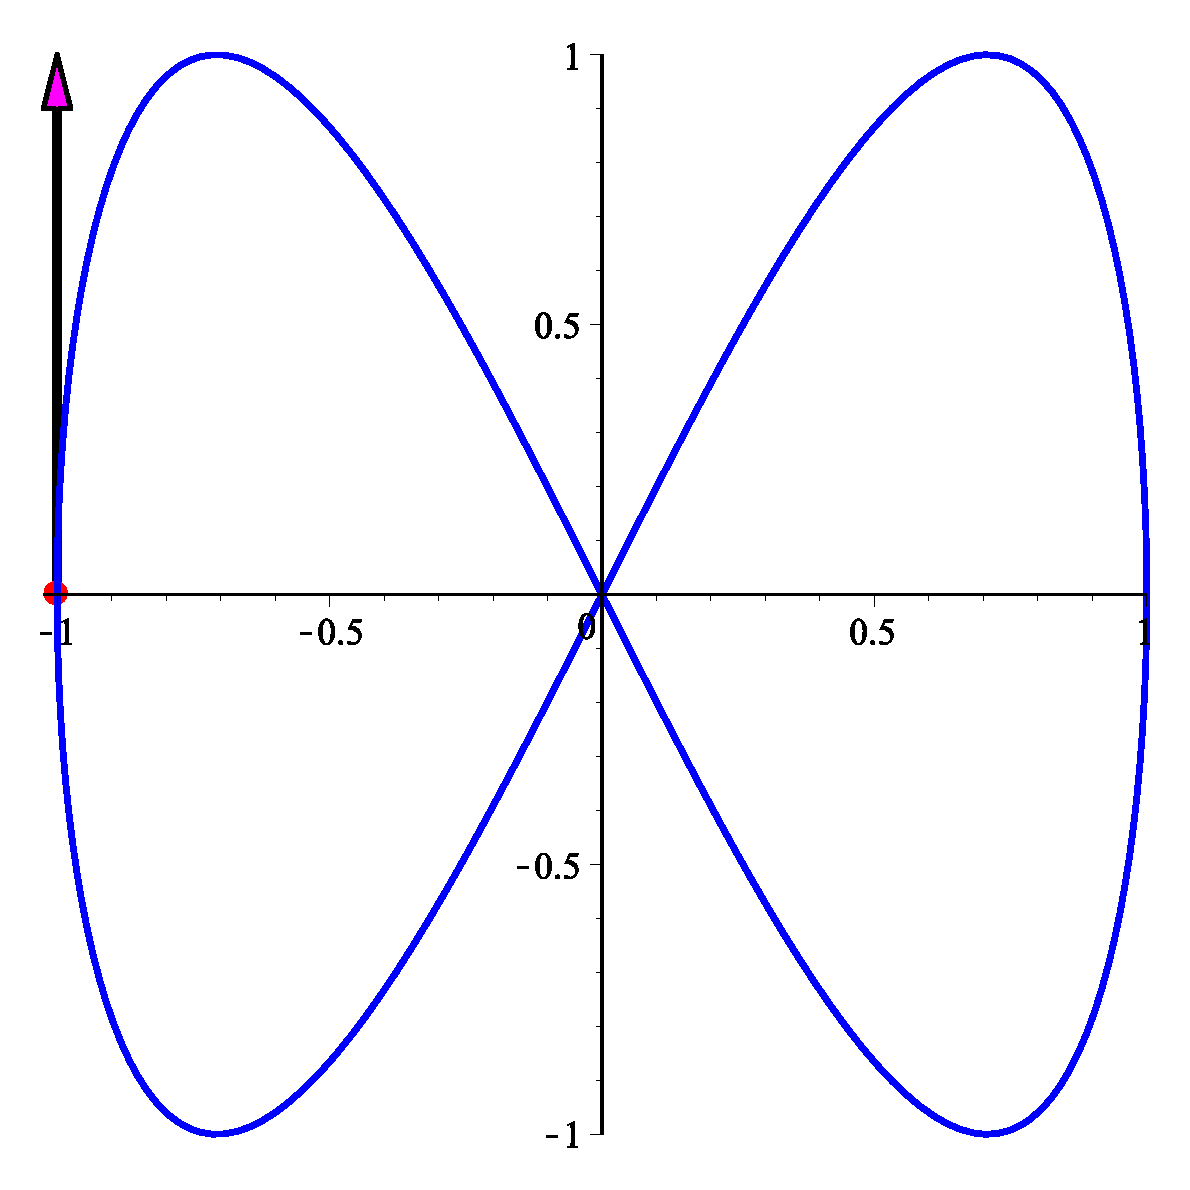
\includegraphics{fig_9_7_PA_b}}
\end{center}
    \ea

\end{activitySolution}

\afterpa 